% Created 2015-06-30 Tue 12:26
\documentclass[captions=tableheading]{scrreprt}
\usepackage[english, ]{babel}
\usepackage{fontspec}
\usepackage{algorithmic}
\usepackage{color}
\usepackage[bookmarks=true]{hyperref}
\hypersetup{linkcolor=blue,filecolor=red,urlcolor=cyan,colorlinks=true}
\usepackage{epstopdf}
\usepackage{graphicx} 
\usepackage{longtable}
\setromanfont{Gentium Basic}
\setromanfont [BoldFont={Gentium Basic Bold},
                ItalicFont={Gentium Basic Italic}]{Gentium Basic}
\setsansfont{Charis SIL}
\setmonofont[Scale=0.7]{DejaVu Sans Mono}
\usepackage{geometry}
\geometry{a4paper, textwidth=130mm, textheight=240mm,
            marginparsep=5mm, marginparwidth=100mm}

\usepackage[yyyymmdd,hhmmss]{datetime}
\renewcommand{\dateseparator}{-}

\pagestyle{headings}

\setlength\parindent{0pt}

\publishers{\tiny\ Compiled on \today\ at \currenttime}

\title{}
      

\usepackage{paralist}
\usepackage{amssymb}
\let\itemize\compactitem
\let\description\compactdesc
\let\enumerate\compactenum
\author{Markus Fix}
\date{2015-06-26}
\title{Aldebaran \\ A High Performance Distributed Processing Environment}
\hypersetup{
 pdfauthor={Markus Fix},
 pdftitle={Aldebaran \\ A High Performance Distributed Processing Environment},
 pdfkeywords={Elemica 2.0},
 pdfsubject={High Performance Distributed Processing},
 pdfcreator={Emacs 24.4.51.2 (Org mode 8.3beta)}, 
 pdflang={English}}
\begin{document}

\maketitle
\tableofcontents

\listoffigures

\chapter{Preamble}
\label{sec:orgheadline1}
This document serves as a record of an iterative design process. It is
\emph{not} a complete specifiation of the system we need to build. We cycle
through multiple iterations as we refine our understanding of the
challenge and contemplate possible designs.

\chapter{The Challenge}
\label{sec:orgheadline8}
\section{Design a streaming data processing system}
\label{sec:orgheadline2}
We are asking you to design a streaming data processing system. You
have as much time as you want to complete the exercise. Final product
should include some kind of design document of the individual
components in the system and how they interact. Where you feel it
necessary, feel free to supply code to illustrate your point. If you
are designing for the use of specific technologies, algorithms etc,
please be sure to indicate. Please address as part of your final work
any tradeoffs you made between requirements and which ones you ended
up favoring.

\section{Application}
\label{sec:orgheadline3}
Our application consumes messages representing financial trade data.
Requests to purchase and purchases. A request to purchase can be
broken down into one or more purchases. In an attempt to get the best
price, the total number of shares purchased can exceed the number
requested. Should the number of shares purchase exceed the requested
amount an alert will be generated.

\section{Example messages}
\label{sec:orgheadline4}
Request to purchase:
\begin{verbatim}
id:1
# shares: 100
client: Sendence
stock: AAPL
\end{verbatim}

Purchase:
\begin{verbatim}
id:2
initial order id: 1
# shares: 90
client: Sendence
stock: AAPL
\end{verbatim}

Purchase:
\begin{verbatim}
id:3
initial order id: 1
# shares: 30
client: Sendence
stock: AAPL
\end{verbatim}

When both purchases 2 and 3 are processed, the number of shares
purchased will exceed the total amount requested in the initial order
and an alert should be generated. Any subsequent purchase shouldn’t
cause any additional alerts.

\section{System Requirements}
\label{sec:orgheadline5}
\begin{itemize}
\item 250,000 msg/sec throughput (with ability to go higher)
\item 5 milliseconds message processing latency
\item System should be able to continue processing in the face of failure
in any individual component
\item Should be usable in both a private datacenter and AWS type
environments
\item Alerts should be received by final intended recipient only once
\item While this exercise is for a specific to a given use case, the
general core of the system should be reusable. When the next use
case comes along, we don’t want to reimplement all the basics over
again.
\end{itemize}

\section{Additional details}
\label{sec:orgheadline6}
\begin{itemize}
\item Source of messages: You can use any message bus you want as entry
point of data into your system so long as it is available as an open
source product (Kafka, RabbitMQ, ActiveMQ). If none of the existing
messaging systems meet the needs of the system, please describe at a
high level the qualities needed for your message bus and roughly how
you might want to implement it.
\item Alerts will be pushed out of our system to any number of downstream
systems, another message bus, to an external alerting/monitoring
system such as Nagios, an SMS messaging provider such as Twilio, as
an iPhone Push Notification or an email. It is the responsibility of
our system to assure only one alert is sent without the ability to
coordinate with the system that provides actual means of delivery.
\item Cost of implementation is a factor. A system that costs \$1 million a
year to run might be worth some tradeoffs with requirements when
compared to a system that costs \$10 million a year to run.
\end{itemize}

\section{Example topics of conversation}
\label{sec:orgheadline7}
\begin{itemize}
\item What message processing guarantees does the system provide?
\item What are the failure characteristics?
\item What are the recovery characteristics?
\item What could cause latency issues?
\item What could cause throughput issues?
\item Are there any single points of failure?
\item What metrics within this system do you consider to be important and
at what points would you want to capture them?
\item What are the monitoring options for each component you’ve specified?
e.g. SNMP, JMX, direct notifications
\item If you’re debating between options for any component in the system,
what are the pros and cons of each and how would you make a final
determination? e.g. Kafka vs RabbitMQ
\end{itemize}


\chapter{Design Process}
\label{sec:orgheadline22}
\section{Iteration 0}
\label{sec:orgheadline11}
We considered if RabbitMq, would scale well
enough for the demanded throughput (250k msg/sec).
A quick search found a \href{http://blog.pivotal.io/pivotal/products/rabbitmq-hits-one-million-messages-per-second-on-google-compute-engine}{study} done by Pivotal where RabbitMq was
scaled to deal with 1 million messages per second. Finding this we
shelved the questions regarding message bus technologies until later.

Let’s start with a naive model of a system that processes the
stream of purchase requests and purchases. We will ignore questions of scaling,
resilience and coordination for now and return to them later.

Figure \ref{fig:orgparagraph1} illustrates the basic message sequence. We
receive a trade data from the TDS into a queue. Our Auditor consumes
trade data and watches the limits for each purchase request. If the
sum of purchases exceeds the defined limit the Auditor publishes an
alert to the Alert Queue. The Fire Lookout consumes alerts from the
Alert Queue and distributes these form to the registered Alert
Channels. Each Alert Channel has it's own Alert Channel Queue which is
processed by a dedicated Channel Boy. The Channel Boy consumes from
the queue and notifies the Alert Channel exactly once for each alert.

\begin{figure}[htb]
\centering
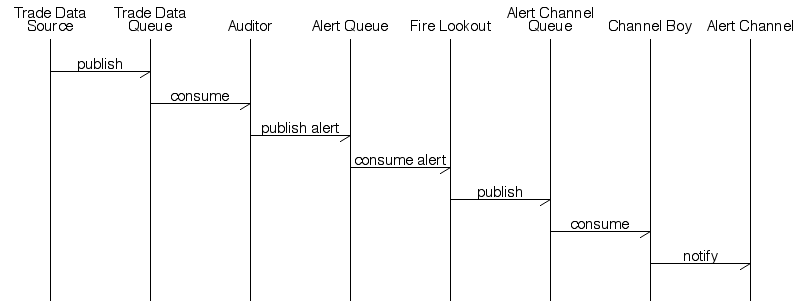
\includegraphics[width=14 cm]{Naive-Flow.png}
\caption{\label{fig:orgparagraph1}
Naive Message Flow}
\end{figure}

\subsection{Assumptions}
\label{sec:orgheadline9}
Some details are underspecified in the challenge description. We've
made the following assumptions:
\begin{enumerate}
\item Events are semi ordered sequences. A purchase request event always
arrives before the related purchase events.
\item We can close an open book (awaiting purchase events) after a
defined delta t or right after we have generated an alert. Once
closed the book can be garbage collected.
\item We do not need to keep a persistent record of books or alerts.
\end{enumerate}

\subsection{Questions}
\label{sec:orgheadline10}
The Auditor will need to keep a book open for each purchase request
to accumulate purchases. 
\begin{enumerate}
\item How will we manage these books in a distributed system?
\item How can we minimize or even eliminate coordination if we run
multiple Auditors to scale up performance?
\item Can we use routing keys to tag each purchase and then route it to
the correct book for accumulation?
\end{enumerate}

\section{Iteration 1}
\label{sec:orgheadline14}
We need to refine the Auditor component. Here's what we know so far:
\begin{enumerate}
\item Each new purchase request event (PR) will open a new book where we
accumulate purchases.
\item Each purchase event (P) will be consumed by the open book and
accumulated.
\item If after accumulating a P the sum of all shares purchased exceeds
our defined limit of the PR the book creates an alert.
\item The alert is published to the Alert Queue.
\end{enumerate}

We introduce two new actors to manage the books and tag incoming
events.

\begin{itemize}
\item The Event Router will notify the Book Manager about incoming PRs. It
tags each event with the PR id it's related to and publishes the
events to the Work Queue.
\item The Book Manager keeps a roster of open books. Once it receives a
notification from the Even Router it will check it's roster. If the
PR id it received from the Event Router is new it will spawn a new
book. The Book Manager starts a timer for each book spawned.
\item Each Book consumes from the work queue.
It only consumes events that are tagged with the PR id each book is
keeping track of. Each Book keeps track of exactly one PR id and
accumulates P events.
\item If the accumulated sum of purchase events P exceed the limit defined
in the PR the Book will publish an alert. After publishing an alert
the Book dies immediately.
\item Once the timer for a Book reaches the defined delta t the Book
Manager sends it a kill command.
\item A Book receiving a kill command finishes any pending processing and then
dies.
\end{itemize}

The Auditor now has three internal actors:
\begin{enumerate}
\item Event Router
\item Book Manager
\item Book
\end{enumerate}

Figure \ref{fig:orgparagraph2} illustrates the even flow between those components.


\begin{figure}[htb]
\centering
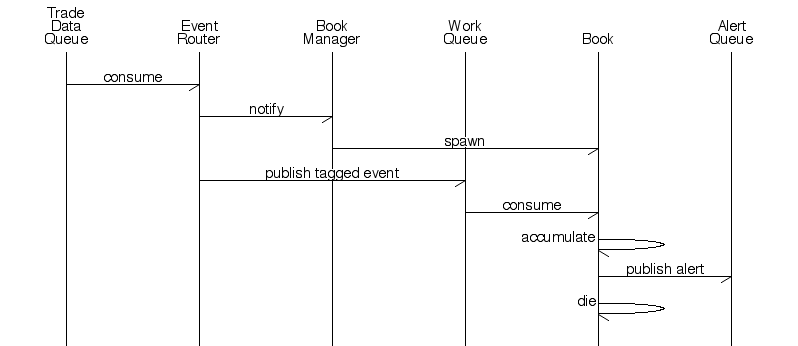
\includegraphics[width=14 cm]{Auditor-1.png}
\caption{\label{fig:orgparagraph2}
Auditor-1}
\end{figure}

Figure \ref{fig:orgparagraph3} shows a system overview with component
interactions.

\begin{figure}[htb]
\centering
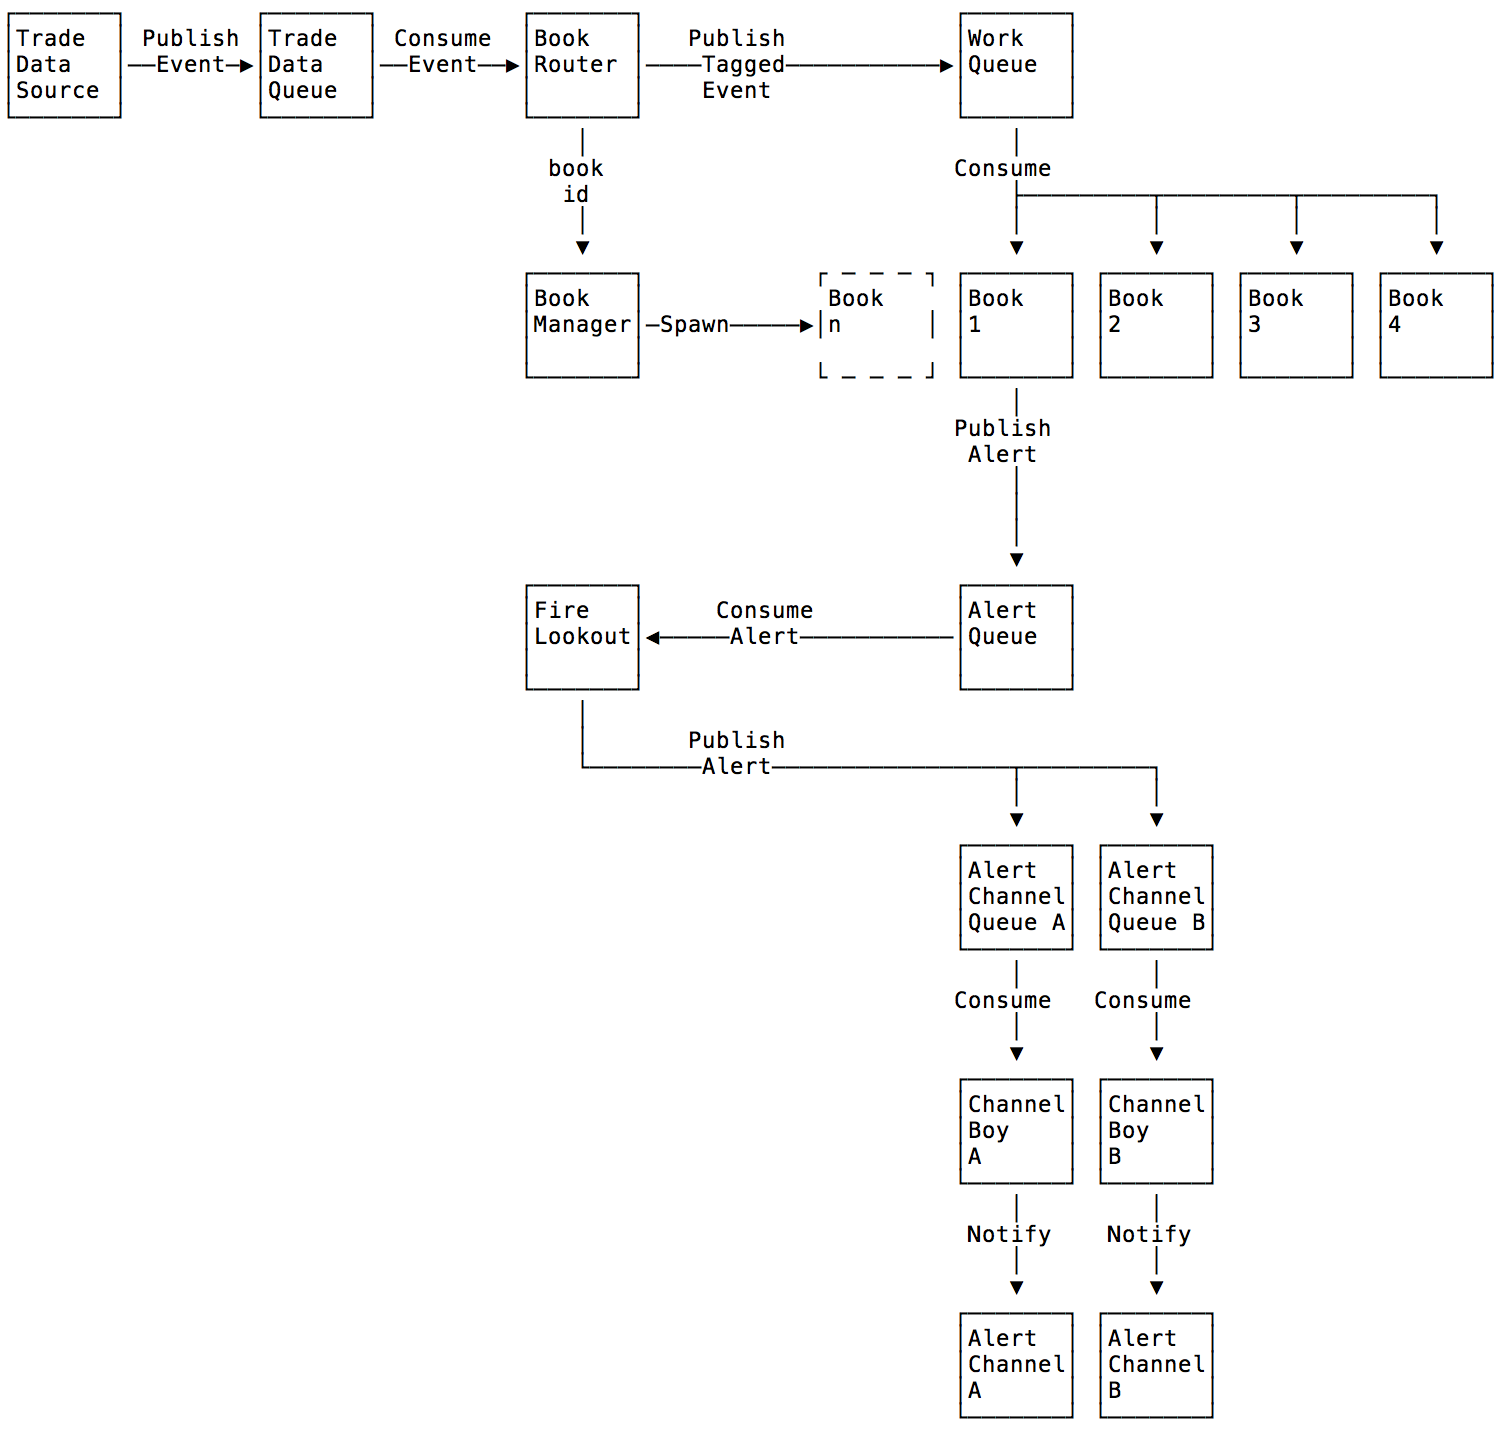
\includegraphics[width=.9\linewidth]{system-overview-1.png}
\caption{\label{fig:orgparagraph3}
System Overview 1}
\end{figure}

\subsection{Questions}
\label{sec:orgheadline12}
\begin{enumerate}
\item How will the Book Router be able to keep up with the message rate?
\item Can we distribute the Book Router?
\item Can we implement the Book Router using a RabbitMq topic exchange?
\item How can we distribute and efficiently manage the creation of books?
\item Books will be very ephemeral. They need an ultra-light process
abstraction?
\item Is routing purchase events P to open books efficiently the key for
achieving optimal throughput?
\item How do we make sure a book does not generate more than one alert?
\item Is it easier to filter duplicates (if any) in the Channel Boy?
\end{enumerate}

\subsection{Assumptions}
\label{sec:orgheadline13}
\begin{enumerate}
\item We do not need to restart books when a book process dies. Meaning
if an open book dies it's state is lost.
\item For now throughput is more important than resilience.
\end{enumerate}

\section{Iteration 2}
\label{sec:orgheadline17}
We now consider the most straightforward way to model the processing
of events by using RabbitMq's routing exchanges.

The Event Router (there can be many) publishes each PR (purchase
request) event to the Purchase Request Exchange. The Purchase Request
Exchange routes each event to the Purchase Request Queue. 

The Event Router (there can be many) implements the following
functionality:
\begin{enumerate}
\item Consume from the Trade Data Queue and publishes PR events to the
Purchase Request Exchange.
\item Consume from the Trade Data Queue and publish P events to the
Purchase Exchange. The Book Router adds a routing header that
contains the PR ID (initial order id). This header is then used
by the Purchase Exchange (a topic exchange) to route the P event to
the correct Purchase Queue.
\end{enumerate}

The Book Manager (there can be many) implements the following
functionality:
\begin{enumerate}
\item Consume the PRs from the Purchase Request Queue.
\item Check if a Purchase Queue with name \texttt{PQ-<PR ID>} already exists.
\item If a Purchase Queue with that name does not exist:
\begin{itemize}
\item Declare a new Purchase Queue with a name like \texttt{PQ-<PR ID>}.
\item Create a binding with \texttt{<PR ID>} as routing key between the
Purchase Exchange and the new Purchase Queue.
\item Spawn a Book.
\end{itemize}
\end{enumerate}

The Book implements the following functionality:
\begin{enumerate}
\item Starts a timer at birth.
\item Subscribes to the Purchase Queue name \texttt{PQ-<PR ID>}.
\item Consumes P events and accumulates the number of purchased shares.
\item If the sum of all accumulated shares exceeds the limit defined for
a PR the Book publishes an alert to the Alert Exchange.
\item Once the timer runs out it unsubscribes from the Purchase Queue and
dies.
\end{enumerate}

The functionality for the Event Router, Book Manager and Book live
inside a component name Auditor. We can spawn multiple Auditors on
multiple distributed nodes. All interactions between components are
via queued messages. The Book Manager spawns Books but they auto
terminate and no pruning or restart logic is necessary.

Figure \ref{fig:orgparagraph4} illustrates the event flow of this design.

\begin{figure}[htb]
\centering
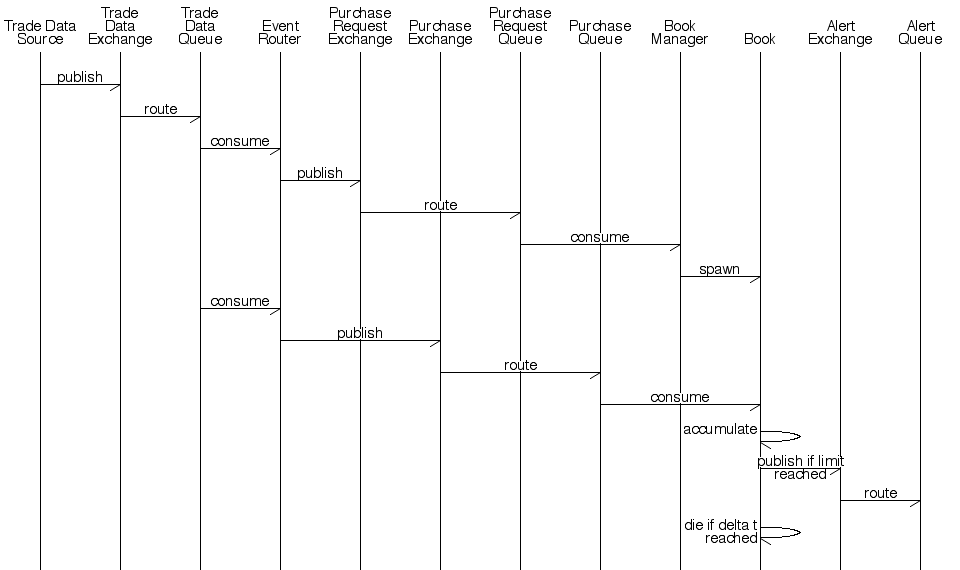
\includegraphics[width=14 cm]{Auditor-2.png}
\caption{\label{fig:orgparagraph4}
Auditor-2}
\end{figure}

Figure \ref{fig:orgparagraph5} shows the updated system overview with component
interactions.

u\begin{figure}[htb]
\centering
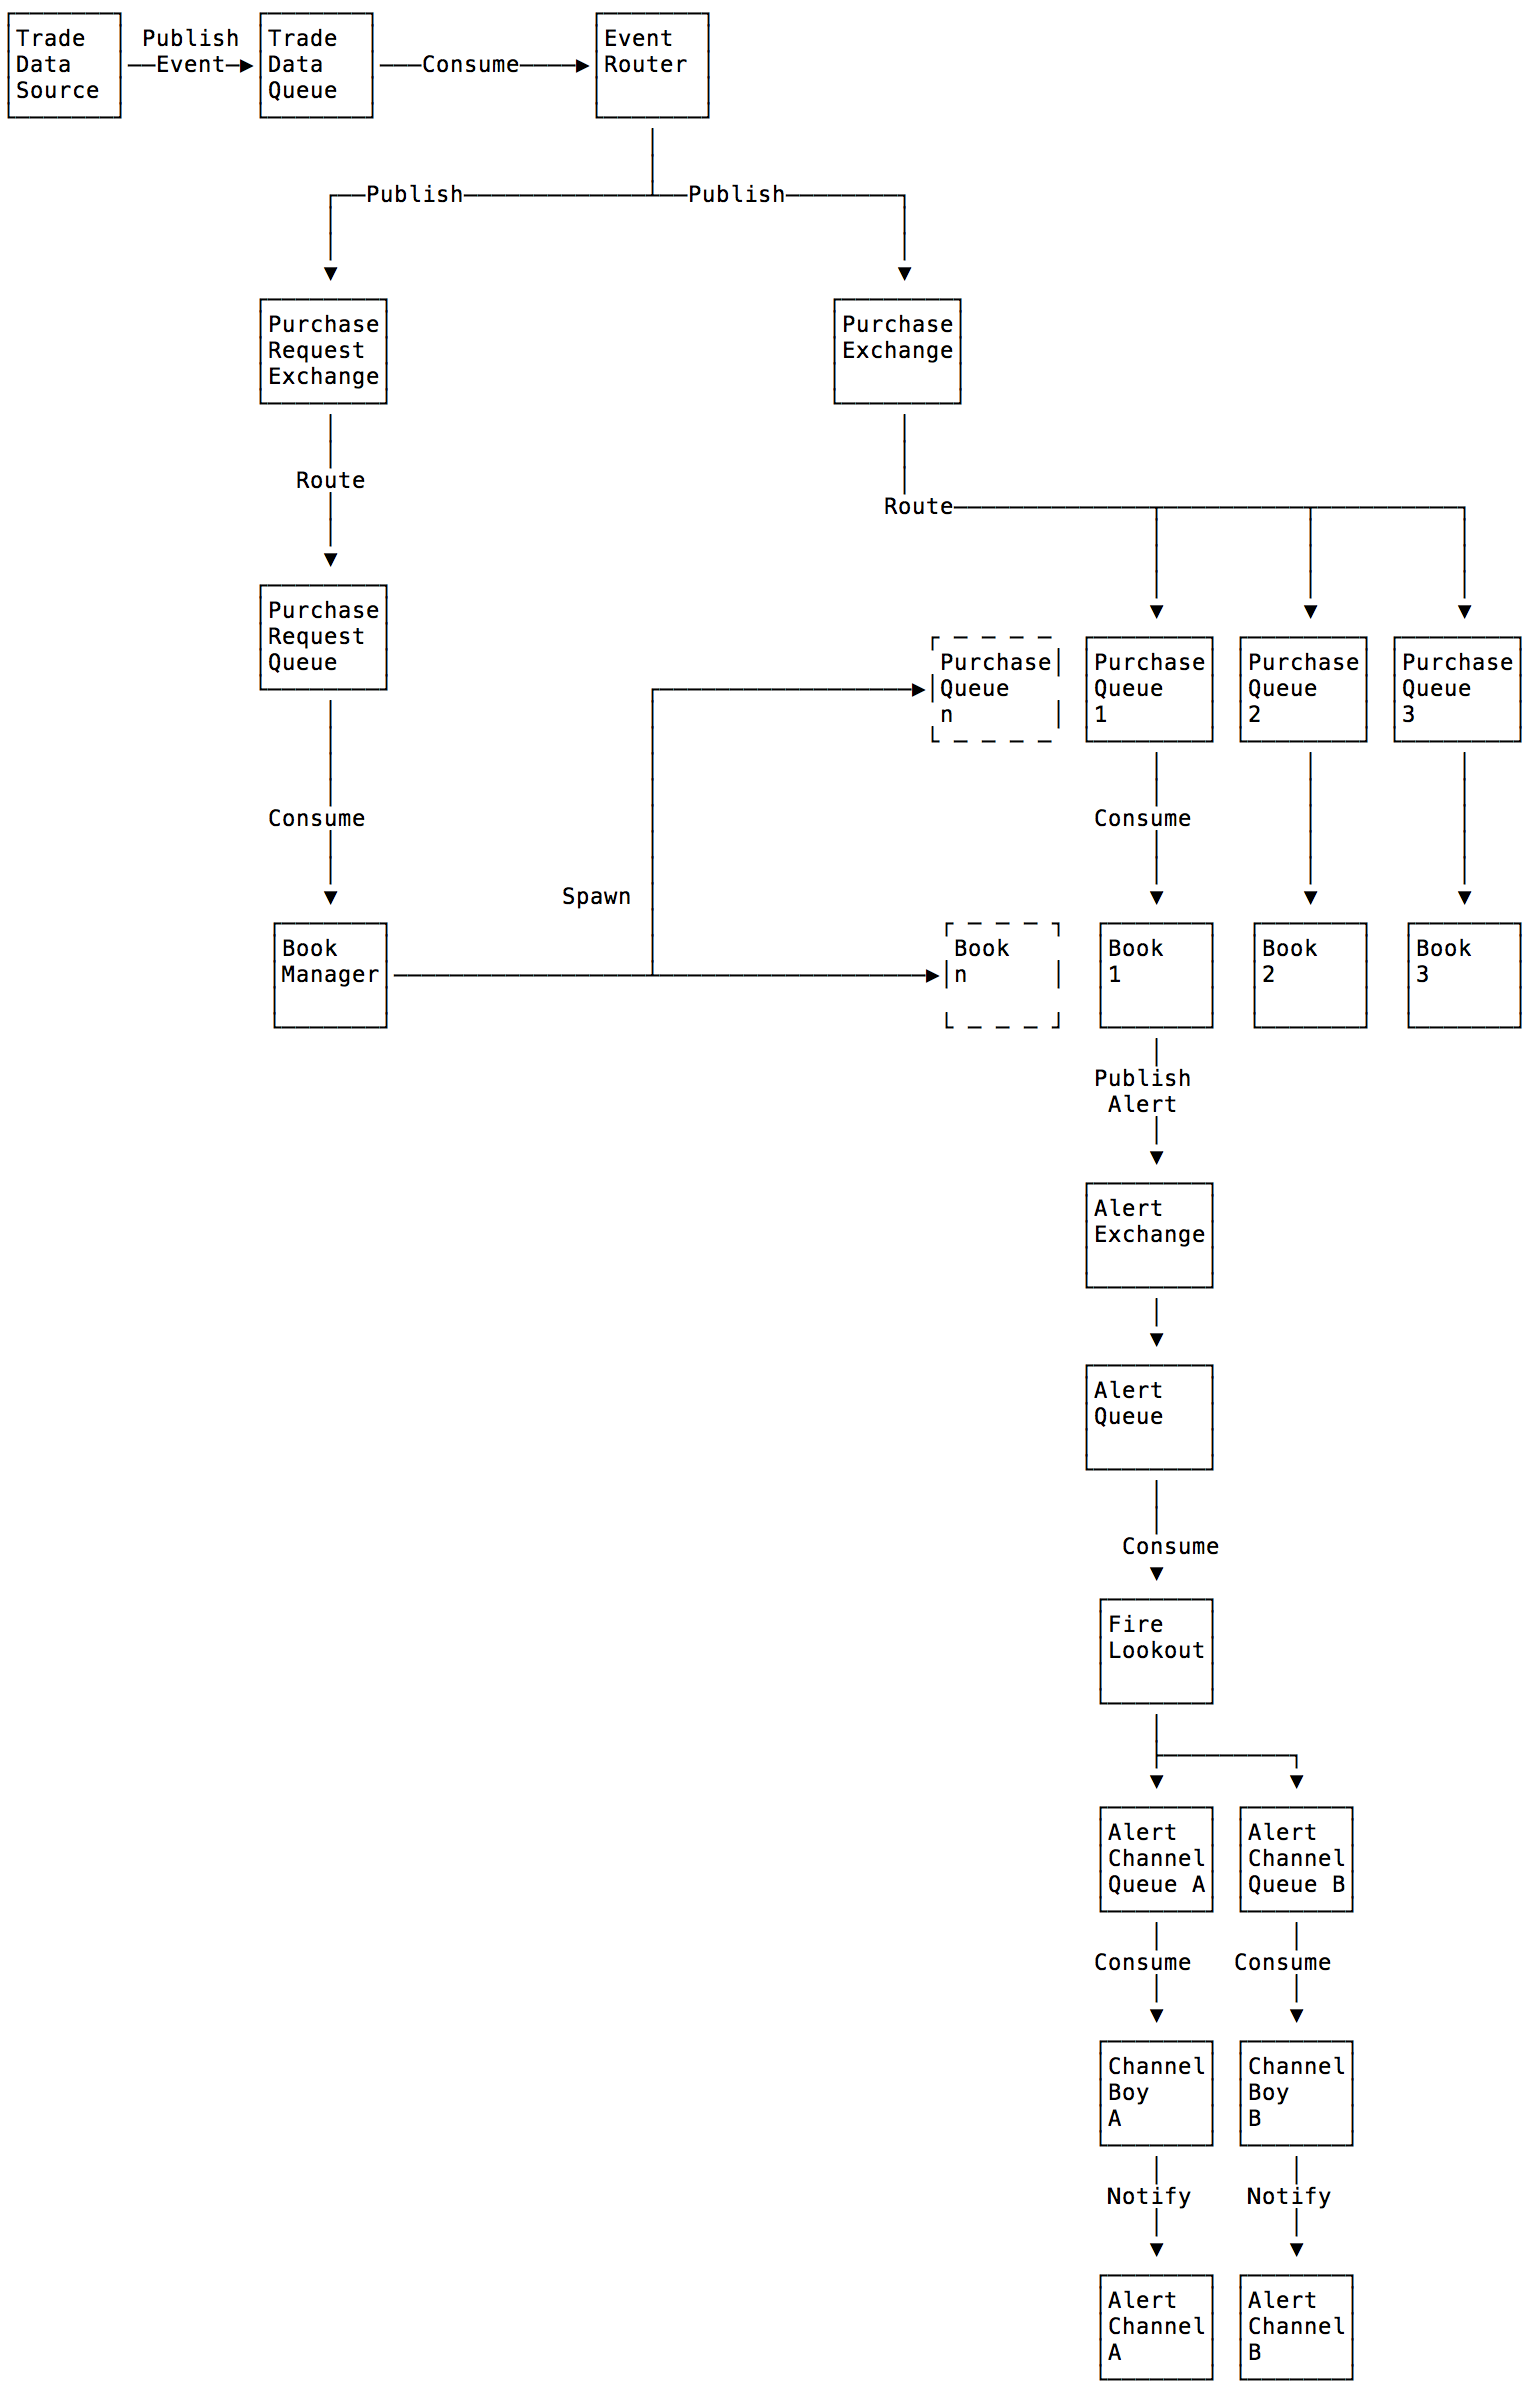
\includegraphics[width=.9\linewidth]{system-overview-2.png}
\caption{\label{fig:orgparagraph5}
System Overview 2}
\end{figure}

\subsection{Assumptions}
\label{sec:orgheadline15}
\begin{enumerate}
\item Events are semi ordered sequences. A purchase request event always
arrives before the related purchase events. This might not be true.
\end{enumerate}

\subsection{Questions}
\label{sec:orgheadline16}
\begin{enumerate}
\item To reduce churn with queue creation / destruction maybe we should
have one Purchase Queue per stock symbol? How would that affect
management of books?
\item None of the queues will survive a broker restart. Is that problematic?
\item There is a potential race condition when a P event arrives before
we've created the Purchase Queue. How can we avoid that?
\item Can we automatically clean up the Purchase Queues if we set them to
auto-delete? That would be removed them automatically once the Book
unsubscribes.
\end{enumerate}


\section{Iteration 3}
\label{sec:orgheadline21}
We need to prepare the development environment as described in section
\ref{sec:orgheadline18} and section \ref{sec:orgheadline19}.

Create the environment:

\begin{verbatim}
mkdir $HOME/aldebaran
cd $HOME/aldebaran
mkvirtualenv aldebaran
workon aldebaran
\end{verbatim}

Install the necessary libraries for the project:
\begin{verbatim}
pip install pika
pip install arrow
\end{verbatim}

\subsection{Publisher}
\label{sec:orgheadline20}
We start with a very simple publisher process. To simplify initial
debugging we publishes with a frequency of 1Hz.

\begin{verbatim}
# This file was auto-generated via org-babel-tangle in Emacs
# Do not modify this file manually. Instead modify the source
# in sendence.org and re-run org-babel-tangle
#
# Usage: ./publisher.py -s localhost 
#

import pika
import uuid
import arrow
import time
import sys
import argparse

def publish(channel, document):
    fields = {}
    fields['uuid'] = str(uuid.uuid4())
    utc = arrow.utcnow().format('YYYY-MM-DDTHH:mm:ssZZ')
    fields['timestamp'] = utc
    channel.basic_publish(exchange='thalys',
                      routing_key='hello',
                      body=document,
                      properties=pika.BasicProperties(headers=(fields)))
    #print " [%s] Sent document" % (utc)
    sys.stdout.write(".")
    sys.stdout.flush()

def main():
    parser = argparse.ArgumentParser(
             description='Loop sending a document to RabbitMq with 1s delay.')
    parser.add_argument('-s', metavar='rabbitmq', default='localhost',
                        help='The IP or DNS name of the RabbitMq server')
    args = parser.parse_args()
    myrabbit = args.s
    myfile = args.f
    # connect to RabbitMq
    try:
        connection = pika.BlockingConnection(
                     pika.ConnectionParameters(host=myrabbit,heartbeat_interval=20))
    except Exception as err:
        print('Cant connect to RabbitMq. Reason: %s' % err)
        exit(1)
    channel = connection.channel()
    # read in the document we want to send
    txt = open(myfile)
    document = txt.read()
    print 'Sending %s to RabbitMq server. To exit press CTRL+C.' % (myfile, )
    while ( 1 ):
        publish(channel, document)
        time.sleep( 1 )
    channel.close()
    connection.close()


if __name__ == "__main__":
    main()
\end{verbatim}


\chapter{Open Questions}
\label{sec:orgheadline23}
\begin{itemize}
\item Scaling Up
\item Resilience
\item Minimizing Coordination
\item Deploy / Release Tooling
\item Live Debugging/ Patching
\item Distributed Monitoring
\end{itemize}

\chapter{Appendix}
\label{sec:orgheadline31}
\section{Setup RabbitMq}
\label{sec:orgheadline18}
We describe the necessary steps to prepare an environment on OSX for
RabbitMq. More information regarding the Firehose Tracer can be found
here: \href{https://www.rabbitmq.com/firehose.html}{Tracer}

The Firehose Tracer enables the tracing of all messages that get
published to exchanges and are consumed from queues.

\subsection{Install RabbitMq}
\label{sec:orgheadline24}
\begin{verbatim}
brew update
brew install rabbitmq
ln -sfv /usr/local/opt/rabbitmq/*.plist ~/Library/LaunchAgents
launchctl load ~/Library/LaunchAgents/homebrew.mxcl.rabbitmq.plist
\end{verbatim}

\subsection{Activate RabbitMq Admin Plugin}
\label{sec:orgheadline25}
\begin{verbatim}
rabbitmq-plugins enable rabbitmq_management
\end{verbatim}

\subsection{Activate the Firehose Trace}
\label{sec:orgheadline26}
Keep in mind that activating tracing is not presistent. If the server
goes down or gets restarted we need to activate tracing again.

\begin{verbatim}
rabbitmqctl trace_on
rabbitmqctl list_exchanges
\end{verbatim}

Activate plugin:
\begin{verbatim}
rabbitmq-plugins enable rabbitmq_tracing
rabbitmq-plugins list
\end{verbatim}

\section{Setup Python Environment}
\label{sec:orgheadline19}
Install git-core:

\begin{verbatim}
brew install git
\end{verbatim}

\subsection{Install Virtualenv}
\label{sec:orgheadline27}
Execute the following commands:

\begin{verbatim}
brew install python --framework
pip install --upgrade pip setuptools
pip install --upgrade virtualenv
mkdir ~/.virtualenvs
pip install --upgrade virtualenvwrapper
\end{verbatim}

\subsection{Install Realpath}
\label{sec:orgheadline28}
The current \texttt{virtualenv} has a dependency on \texttt{realpath} that is not
satisfied on OSX. Do the following to fix this:

\begin{verbatim}
brew tap iveney/mocha
brew install realpath
\end{verbatim}

\subsection{Configure}
\label{sec:orgheadline29}
Add the following to \texttt{\$HOME/.bash\_profile} or \texttt{\$HOME/.zprofile}:

\begin{verbatim}
export VIRTUALENVWRAPPER_PYTHON=/usr/local/bin/python
export WORKON_HOME=~/.virtualenvs
source /usr/local/bin/virtualenvwrapper.sh
\end{verbatim}


\section{RabbitMq Tuning}
\label{sec:orgheadline30}
RabbitMQ's queues are fastest when they're empty. When a queue is
empty, and it has consumers ready to receive messages, then as soon as
a message is received by the queue, it goes straight out to the
consumer. In the case of a persistent message in a durable queue, yes,
it will also go to disk, but that's done in an asynchronous manner and
is buffered heavily. The main point is that very little book-keeping
needs to be done, very few data structures are modified, and very
little additional memory needs allocating. \href{http://www.rabbitmq.com/blog/2011/10/27/performance-of-queues-when-less-is-more/}{Performance of Queues}

The main factor is consumer performance. Keep those queues empty!
\end{document}